Neste capítulo será apresentada a proposta de aceleração da operação de verificação de dominância
através da utilização da \kdtree{} como estrutura de indexação multidimensional de soluções.
Para isso, as duas variações da operação de verificação de dominância e suas
interpretações como problema de busca de faixa serão definidas.
A utilização da \kdtree{} será também comparada a da lista encadeada e a da árvore AVL.

\section{A Verificação de Dominância e a Busca de Faixa}

Como dito anteriormente, solucionar um problema multiobjetivo significa
apresentar o seu \paretoset{}, ou seja, o conjunto de soluções que
não são dominadas por nenhuma outra.
Geralmente o \paretoset{} é construído pelos algoritmos de forma incremental, ou seja,
através da adição progressiva de soluções candidatas.
Por este motivo, um dos procedimentos mais executados durante o processo de solução
é o de verificar se uma determinada solução é dominada por alguma outra
pertencente a um \paretoset{} candidato.

Um algoritmo também pode necessitar reduzir um conjunto de soluções
a um conjunto independente, ou seja, conjunto no qual nenhuma das soluções é dominada por
alguma outra do mesmo conjunto, o que demanda esforço quadrático sobre o número de soluções,
se implementado como uma comparação par a par.
Entretanto, se as soluções forem interpretadas como pontos em um espaço
multi-dimensional, pode-se deduzir, da Equação~\ref{eq:dom}, que este tipo de verificação
corresponde ao problema de verificação de existência de pontos em uma determinada
região retangular do espaço.
Este problema é conhecido por alguns ramos da computação e é denominado \emph{busca de faixa}
(\emph{range search} em inglês).
%As Figuras~\ref{img:pnt-reg} e \ref{img:pnt-reg-minus} ilustram os casos
%mencionados.

\begin{figure}[!ht]
  \centering
  \begin{minipage}[b]{0.42\textwidth}
    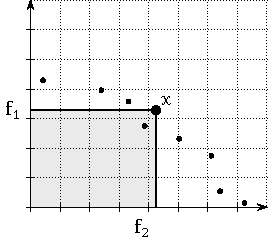
\includegraphics[width=\textwidth]{img/mokp/pnt-reg}
    \caption{Verificação da existência de solução dominada por $x$.}
    \label{img:pnt-reg}
  \end{minipage}
  \hfill
  \begin{minipage}[b]{0.42\textwidth}
    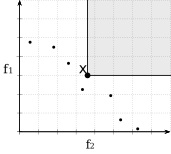
\includegraphics[width=\textwidth]{img/mokp/pnt-reg-minus}
    \caption{Verificação da existência de solução que domine $x$.}
    \label{img:pnt-reg-minus}
  \end{minipage}
\end{figure}

A Figura~\ref{img:pnt-reg} ilustra o primeiro caso do problema de verificação de dominância:
determinar se, dentre um conjunto de soluções, existe alguma que é dominada por uma solução $x$.
O problema é equivalente ao de verificar se existe algum ponto na região sombreada,
correspondente à região dominada pela solução $x$.
No caso, existe uma solução que é dominada por $x$.

A Figura~\ref{img:pnt-reg-minus} ilustra o segundo caso do problema de verificação de dominância:
determinar se, dentre um conjunto de soluções, existe alguma que domina a solução $x$.
O problema é equivalente ao de verificar se existe algum ponto na região sombreada,
correspondente à região que domina a solução $x$.
No caso, não existe nenhuma solução.

Para que seja devidamente formalizado o mapeamento entre o problema de verificação
de dominância e o problema de busca de faixa, é necessário primeiramente definir
duas regiões do espaço, referentes às áreas de interesse neste tipo de operação.
Define-se a área $R_d(x)$ dominada pela solução $x$ e a área $R_{d-}(x)$ a qual domina
a solução $x$ sendo respectivamente:
\begin{align*}
  R_d(x) &= \big\{y \in \mathbb{R}^\np \;\big|\; y_i \leq f_i(x), i \in \{1, \ldots, \np\}\big\}\\
  R_{d-}(x) &= \big\{y \in \mathbb{R}^\np \;\big|\; y_i \geq f_i(x), i \in \{1, \ldots, \np\}\big\}
\end{align*}
\noindent As Figuras~\ref{img:dom-reg} e \ref{img:dom-reg-minus} ilustram as
regiões definidas.

\begin{figure}[!ht]
  \centering
  \begin{minipage}[b]{0.42\textwidth}
    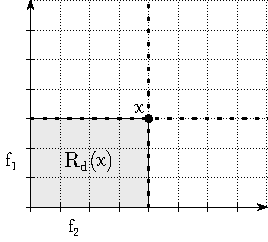
\includegraphics[width=\textwidth]{img/mokp/dom-reg}
    \caption{Região $R_d(x)$ dominada pela solução $x$.}
    \label{img:dom-reg}
  \end{minipage}
  \hfill
  \begin{minipage}[b]{0.42\textwidth}
    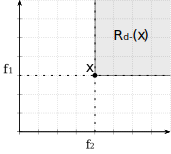
\includegraphics[width=\textwidth]{img/mokp/dom-reg-minus}
    \caption{Região $R_{d-}(x)$ pela qual a solução $x$ é dominada.}
    \label{img:dom-reg-minus}
  \end{minipage}
\end{figure}

Pode-se então definir, por exemplo, para um caso par a par, que o problema de verificar se uma
solução $x$ domina uma solução $y$ é equivalente ao problema de verificar se
o ponto $f(y)$ está contido na região $R_d(x)$, ou seja:
\begin{displaymath}
    x \dom y \; \Leftrightarrow \; \pnt{y} \in R_d(\sol{x})
\end{displaymath}
\noindent Para a primeira variação do problema, verificar se, dentre um conjunto $Y$
de soluções, existe alguma solução $y \in Y$ dominada por $x$ (Figura~\ref{img:pnt-reg}) equivale ao problema de
determinar se algum ponto está contido na região $R_d(x)$. Formalmente:
\begin{displaymath}
  \exists(y \in Y)[\; x \dom y \;] \; \Leftrightarrow \;
    \exists(y \in Y)[\;f(y) \in R_{d}(x)\;]
\end{displaymath}
\noindent Semelhantemente, o problema de verificar se, dentre um conjunto $Y$
de soluções, existe alguma solução $y \in Y$ que domina uma solução $x$ (Figura~\ref{img:pnt-reg-minus}) equivale ao
problema de verificar se existe algum ponto $f(y)$ contido na região $R_{d-}(x)$.
Formalmente:
\begin{align*}
  \exists(y \in Y)[\; y \dom x \;] \; \Leftrightarrow \;
    \exists(y \in Y)[\;f(y) \in R_{d-}(x)\;] \\
\end{align*}

O problema de se determinar a existência de um ponto numa determinada região do
espaço é largamente aplicado, por exemplo, na área da
computação gráfica e jogos, onde é necessário verificar a colisão entre pontos e polígonos.
Para auxiliar na solução deste problema, uma das estruturas de dados recomendadas é a \kdtree{}
~\cite{agarwal1999geometric}.
A proposta do presente trabalho é utilizar a \kdtree{} como estrutura auxiliar também
nas operações de verificação de dominância, o que deve acelerar o procedimento,
uma vez que as soluções estarão indexadas por uma estrutura própria para este tipo
de operação.

A seguir são apresentadas três estruturas de dados que podem ser utilizadas para
auxiliar à operação de busca de faixa.
Duas das estruturas, a lista encadeada e a árvore AVL, já são utilizadas pela
literatura no auxílio à verificação de dominância.
A terceira estrutura, a \kdtree{}, será proposta
como estrutura ideal para ser utilizada neste tipo de operação.

\section{Lista Encadeada}

A lista encadeada é uma estrutura de dados na qual cada um dos elementos,
dispostos em ordem linear, possuem um ponteiro que referencia um próximo elemento
~\cite{cormen2009introduction}.
A lista portanto não possui qualquer ordenação ou indexação baseada nos valores dos
elementos.
A sequência em que os elementos são dispostos é definida pela ordem de inserção
dos elementos na lista.
A Figura~\ref{fig:lst-model} apresenta uma lista encadeada contendo 7 números inteiros como elementos.
O ponto ao final de cada estrutura representa o ponteiro para o próximo nó da lista.

\begin{figure}[ht]
  \centering
  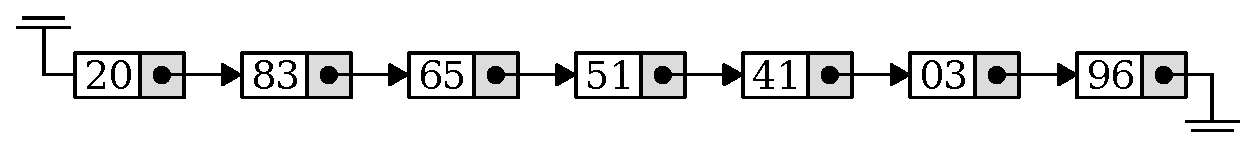
\includegraphics[scale=0.6]{img/kdt/lst-model}
  \caption{Exemplo de lista encadeada contendo 7 elementos.}
  \label{fig:lst-model}
\end{figure}

%Um elemento pode ser inserido em uma lista encadeada mantendo-se a ordem dos elementos
%já existentes, desde que inserido ao final da lista.
%Para que isto seja feito com maior eficiência guarda-se o ponteiro para o
%último elemento da lista.
%A inserção é feita através da atualização do ponteiro mantido pelo último elemento,
%fazendo-o agora referenciar o novo elemento.
%A Figura~\ref{fig:lst-insert} ilustra a inserção do elemento $17$ ao final de uma lista encadeada.

%\begin{figure}[ht]
%  \centering
%  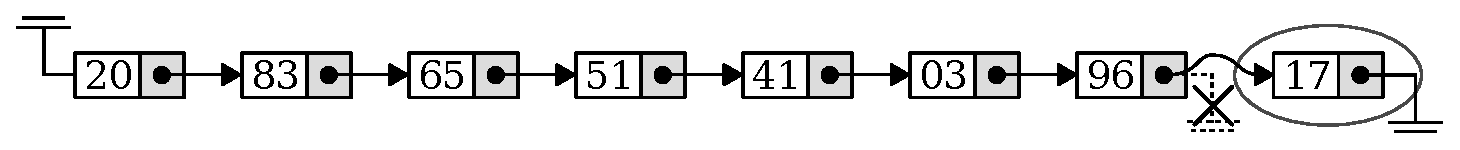
\includegraphics[scale=0.6]{img/kdt/lst-insert}
%  \caption{Operação de inserção de elemento em uma lista encadeada.}
%  \label{fig:lst-insert}
%\end{figure}

%Para realizar a remoção de um elemento é necessário primeiramente localizar o elemento na lista.
%Para isso, parte-se do primeiro elemento da lista e caminha-se elemento a elemento
%até encontrar o desejado.
%Assim que encontrado, a remoção do elemento é feita através da atualização do ponteiro
%do seu antecessor, fazendo-o apontar agora para o que era seu sucessor.
%A Figura~\ref{fig:lst-remove} ilustra a operação de remoção do elemento $41$ de uma lista encadeada.

%\begin{figure}[ht]
%  \centering
%  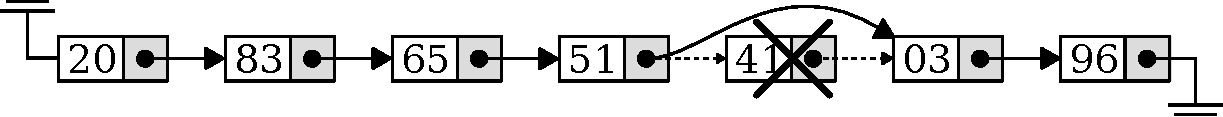
\includegraphics[scale=0.6]{img/kdt/lst-remove}
%  \caption{Operação de remoção de elemento em uma lista encadeada.}
%  \label{fig:lst-remove}
%\end{figure}

Uma vez que a lista encadeada é ``cega'' quanto aos valores dos elementos,
a única forma de realizar uma operação de busca de faixa
é partindo do primeiro da lista e avaliando cada elemento
de forma sucessiva, até encontrar algum que esteja na faixa desejada.
Caso não exista nenhum elemento na faixa desejada, todos os elementos serão avaliados.
O Algoritmo~\ref{alg:alg-range-lst} apresenta o algoritmo de busca
de faixa utilizando uma lista encadeada.

O Algoritmo~\ref{alg:alg-range-lst} inicia considerando o primeiro nó (head) como sendo o nó corrente (node).
Enquanto o nó corrente não é $null$ (linha 3), ou seja, enquanto não
se alcançou o final da lista, o algoritmo
recupera o elemento contido no nó (linha 4) e verifica
se este é um ponto contido em $R_d(x)$ (linha 5).
Em caso verdadeiro, é retornado o elemento (linha 6).
Caso contrário, o algoritmo segue para o próximo nó da
lista (linha 7) até alcançar o final da lista.

\begin{algorithm}
  \Kw{$x$: ponto de interesse, $L$: lista de pontos}
\Begin{
  $\texttt{node} \gets \texttt{L.head}$\;
  \While{\texttt{node} $\neq null $}{
    $y \gets \texttt{node.info}$\;
    \If{$y \in R_d(x)$}{
      \textbf{return} $y$\;
    }
    $\texttt{node} \gets \texttt{node.next}$
  }
  \textbf{return} null\;
}
  \caption{Procedimento busca de faixa utilizando pontos mantidos por uma lista encadeada.}
  \label{alg:alg-range-lst}
\end{algorithm}

A Figura~\ref{img:pts-lst-model} apresenta pontos dispostos em um plano,
mantidos por uma lista encadeada.
No plano pode-se notar o retângulo com bordas pontilhadas, representando a região
de interesse para a qual se deseja consultar a pertinência de algum ponto.
A Figura~\ref{img:pts-lst-query} ilustra a execução da busca de faixa.
O fundo cinza sob o ponto sinaliza a avaliação do ponto.
No exemplo, apenas o ponto $26$ está contido no intervalo de busca.
Porém, dos $27$ pontos, foi necessário avaliar os $22$ pontos que estavam
armazenados nas posições anteriores ao ponto $26$.

\begin{figure}[ht]
  \centering
  \begin{minipage}[t]{0.48\textwidth}
    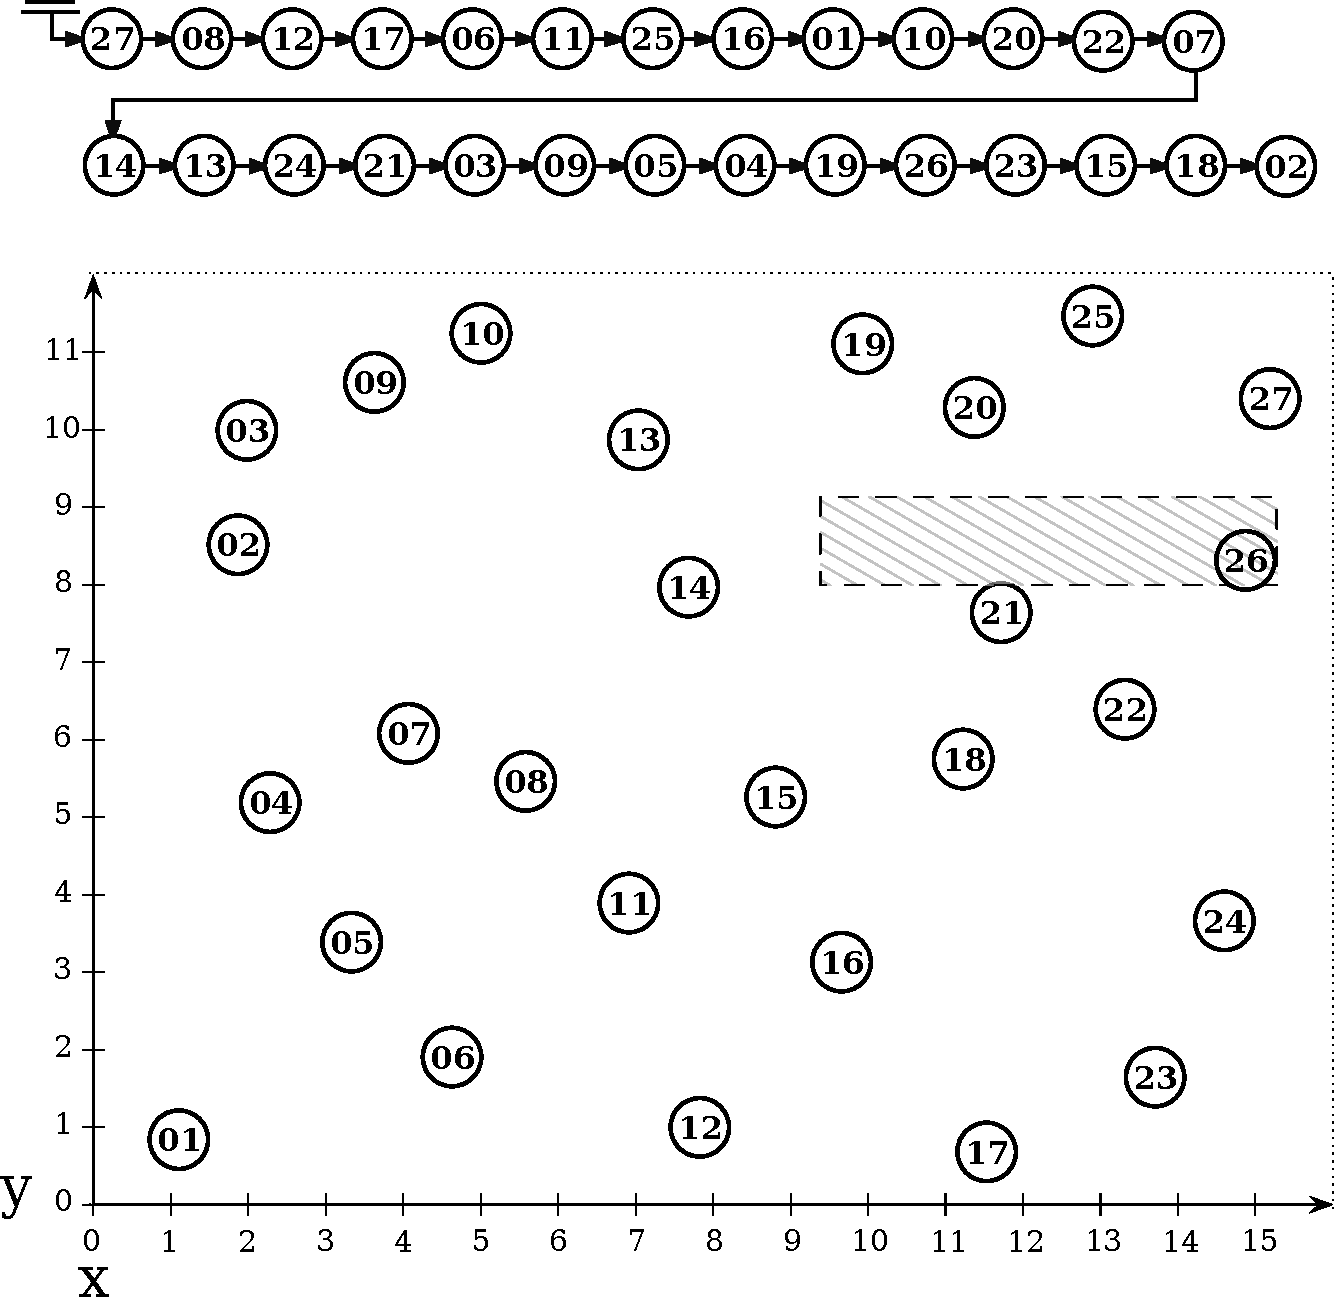
\includegraphics[width=\textwidth]{img/points-query/lst/points-lst-model}
    \caption{Pontos no plano mantidos por uma lista encadeada.}
    \label{img:pts-lst-model}
  \end{minipage}
  \hfill
  \begin{minipage}[t]{0.48\textwidth}
    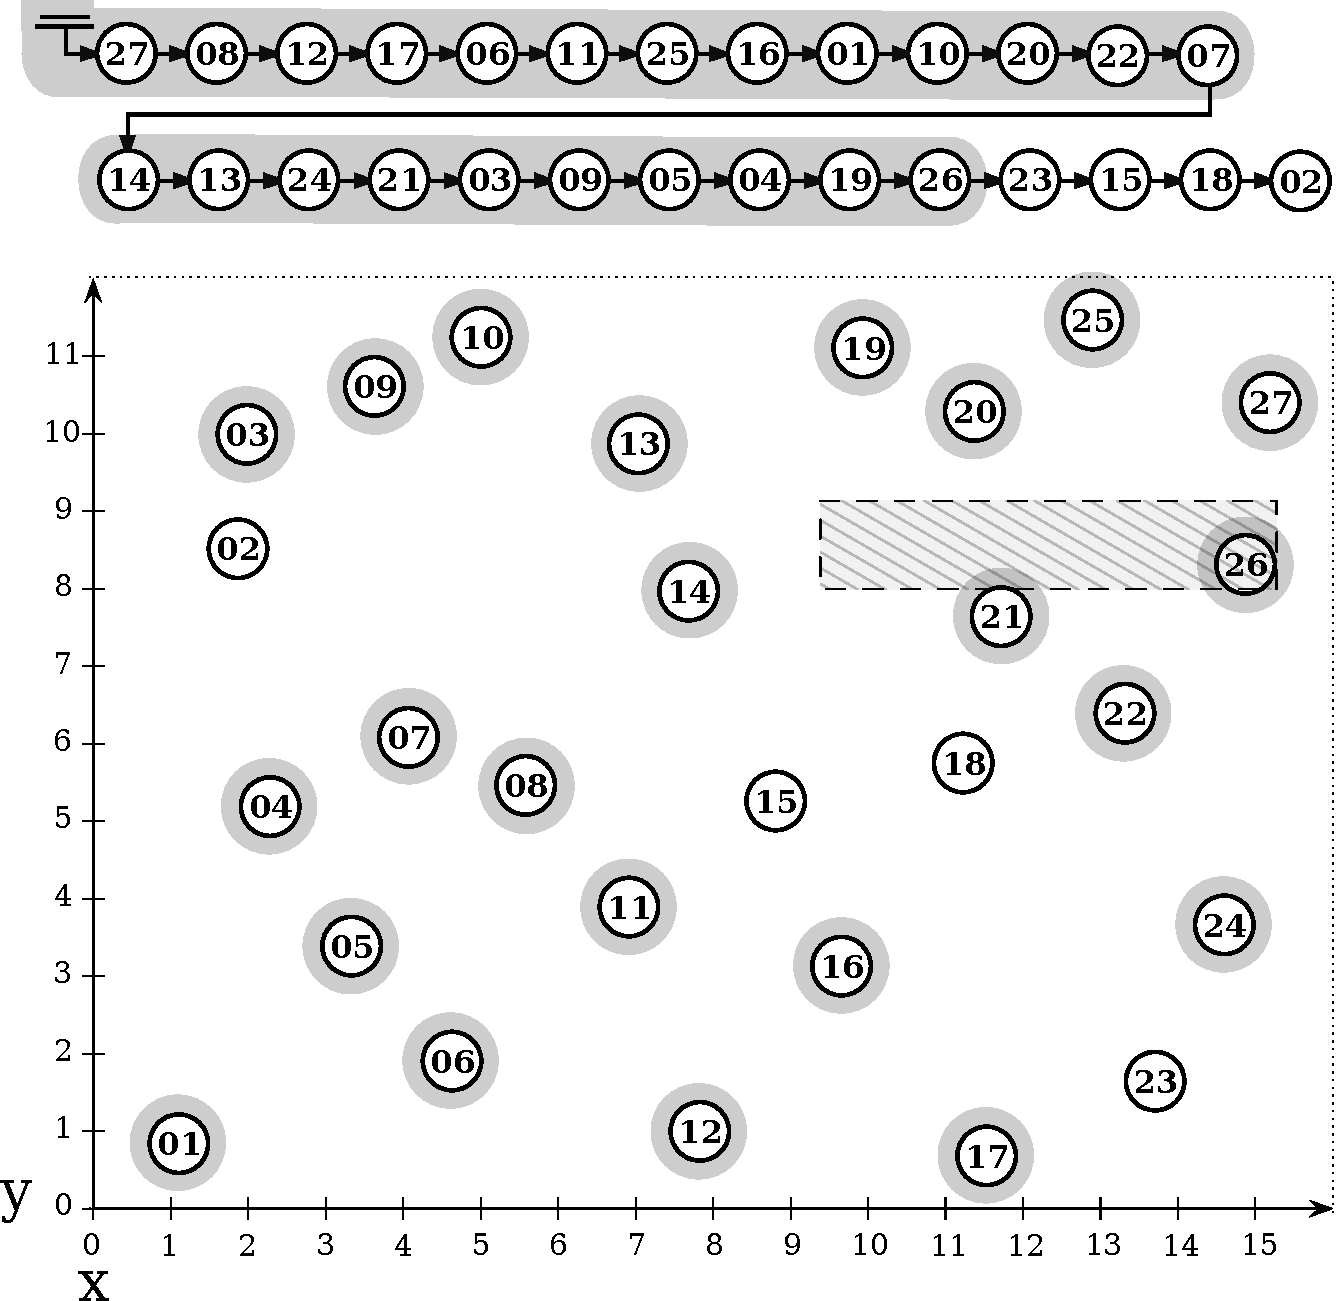
\includegraphics[width=\textwidth]{img/points-query/lst/points-lst-query}
    \caption{Execução da operação de busca de faixa em pontos mantidos por uma lista encadeada.}
    \label{img:pts-lst-query}
  \end{minipage}
\end{figure}



\section{Árvore AVL}

A árvore AVL é um tipo de árvore binária de busca com a propriedade de ter sua altura
\emph{balanceada}, ou seja, proporcional ao logaritmo do número total de elementos.
Para alcançar esse balanceamento a árvore AVL assegura que, para cada nó da árvore,
a diferença de altura entre as sub-árvores da esquerda e da direita seja no máximo $1$.
Esse balanceamento é independente da ordem em que os elementos são inseridos
ou removidos, o que garante eficiência nas operações de busca.

Para que as operações de inserção e remoção de elementos sejam feitas de forma eficiente,
é necessário que cada nó mantenha informação sobre o
balanceamento entre as suas sub-árvores.
Assim, as operações de inserção e remoção de elementos podem ser executadas de forma
eficiente, mantendo-se a estrutura balanceada da árvore, realizando,
sempre que necessário, operações de reposicionamento dos nós \emph{pais}.

A Figura~\ref{fig:avl-model} apresenta uma árvore AVL contendo 7 números
inteiros como elementos, tendo o elemento 65 como nó raiz.
A parte branca de cada nó representa a informação contida, enquanto que a
parte cinza representa dados estruturais da árvore.
Cada nó possui espaço para guardar duas referências para nós filhos: um
à direita e outro à esquerda.
Como qualquer árvore binária de busca, os elementos dispostos à esquerda de um nó são sempre menores que o elemento mantido pelo nó e os elementos dispostos à direita são sempre
maiores ou iguais que o elemento mantido pelo nó.
O espaço central da região acinzentada contém a informação do balanceamento da árvore: altura da sub-árvore à direita menos a altura da sub-árvore à esquerda, que pode variar de -1 a +1.

\begin{figure}[ht]
  \centering
  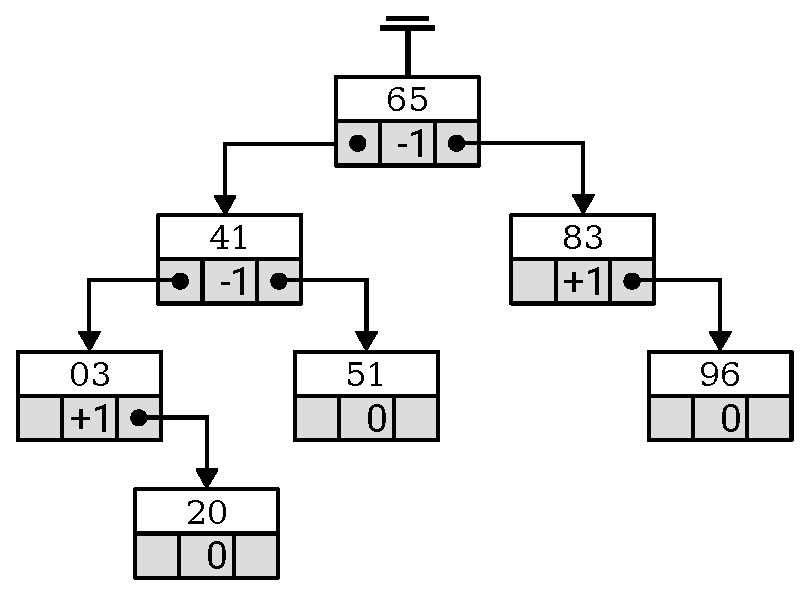
\includegraphics[scale=0.6]{img/kdt/avl-model}
  \caption{Exemplo de árvore AVL contendo 7 elementos.}
  \label{fig:avl-model}
\end{figure}

Vale observar que a árvore AVL, como qualquer outra árvore binária de busca,
mantém uma ordenação crescente dos valores dos elementos, se considerada
uma navegação da esquerda para a direita, priorizando os elementos em níveis inferiores
às sub-árvores.
Tal navegação para a Figura~\ref{fig:avl-model} seria 03, 20, 41, 51, 65, 83 e 96.
O valor que a árvore considera para a ordenação é chamado de \emph{chave}.

A busca por um elemento em uma árvore AVL é feita da mesma maneira
que em uma árvore binária de busca comum.
Primeiramente avalia-se o nó raiz. Caso este seja menor que o elemento buscado,
prossegue-se avaliando a sub-árvore à esquerda, caso contrário, prossegue-se à sub-árvore à direita.
A navegação pelas sub-árvores continua, até que um nó com o mesmo valor buscado
seja encontrado ou até que se encontre um nó sem a sub-árvore a ser avaliada.
Neste último caso, conclui-se que o elemento buscado não existe na árvore.

Para se buscar, por exemplo, o elemento $20$ na árvore da Figura~\ref{fig:avl-model}, inicialmente avalia-se o nó raiz $65$.
Uma vez que $20$ é menor que $65$ a busca prossegue para o nó $41$ à esquerda.
Uma vez que $20$ também é menor que $41$ a busca prossegue para o nó $03$.
Como $20$ é maior que $03$, prossegue-se para a direita, encontrando-se finalmente o elemento $20$ buscado.
Para se buscar, por exemplo, o elemento $84$, serão visitados respectivamente
os nós $65$, $83$ e $96$.
Visto que $84$ é menor que $96$ porém o nó $96$ não possui sub-árvore à esquerda,
a busca se encerra e conclui-se que o elemento $84$ não existe na árvore.

Uma vez que a árvore AVL mantém uma ordenação sobre os valores dos elementos,
é possível realizar uma busca de faixa com uma maior eficiência que em uma lista encadeada.
Porém, convém observar que para se armazenar pontos multidimensionais, a árvore AVL
deve considerar apenas uma das dimensões, que será utilizada como chave.
As demais dimensões serão desconsideradas pela estrutura.
A proposta deste trabalho é que esse fato representa uma potencial deficiência
da estrutura quanto à operação de busca de faixas sobre dados multidimensionais,
especialmente para uma grande quantidade de dados com mais de duas dimensões,
deficiência esta sanada pela \kdtree{}.

Para se realizar uma operação de busca de faixa sobre pontos
armazenados em uma árvore AVL, o primeiro passo é observar os limites da faixa de busca
na dimensão (ou coordenada) utilizada como chave pela árvore, pois a busca
se caracteriza por uma varredura de todos os elementos nos limites nesta dimensão.
A busca prossegue então localizando o elemento que está mais a esquerda na região de busca,
ou seja, que possui o menor valor de chave.
A partir desse elemento então é feita uma varredura dos elementos a direita, ou seja,
em ordem crescente de valor de chave.
Para cada elemento visitado, suas demais coordenadas são verificadas.
A busca se encerra ao encontrar algum elemento na região de interesse ou
caso a região seja extrapolada pela direita.
Neste último caso conclui-se que não existe nenhum elemento na região buscada.

A Figura~\ref{img:pts-avl-model} ilustra  uma árvore AVL
que considera a componente $x$ com chave e guarda
os mesmos 27 pontos das Figuras~\ref{img:pts-lst-model} e \ref{img:pts-lst-query}.
Também apresenta a mesma área de interesse (retângulo pontilhado).
Vale observar a ordenação que a árvore mantém quanto à distribuição dos pontos
ao longo da coordenada $x$.

A Figura~\ref{img:pts-avl-query} ilustra a operação de busca de faixa utilizando
a árvore AVL.
As duas setas acinzentadas no plano indicam a região que a árvore AVL
deve avaliar para verificar a possível pertinência de um ponto na região de busca
(retângulo pontilhado).
Os limites na coordenada $x$ da região de busca são $9,4$ e $15$.
Vale observar que, apesar da região de busca ser um estreito retângulo horizontal,
faz-se necessário verificar os pontos em toda a extensão vertical da região avaliada,
pois a árvore não considera o posicionamento vertical dos pontos.
O fundo cinza sob o ponto sinaliza a avaliação do ponto.
A linha direcionada que percorre a árvore na parte superior da figura indica
a sequência em que os nós são avaliados até encontrar o ponto 26.
O primeiro passo da execução é encontrar o ponto mais à esquerda da região
a ser verificada (ponto 15).
Assim que esse ponto é encontrado, inicia-se a varredura da
região da esquerda para a direita.
Vale observar que durante a varredura, ao se esgotar os nós à esquerda de uma
sub-árvore é necessário ``voltar'' ao nó pai para continuar a
varredura na sub-árvore à direita.
Após avaliar $14$ dos $27$ pontos, é encontrado o ponto 26 pertencente
à região de busca.

\begin{figure}[ht]
  \centering
  \begin{minipage}[t]{0.48\textwidth}
    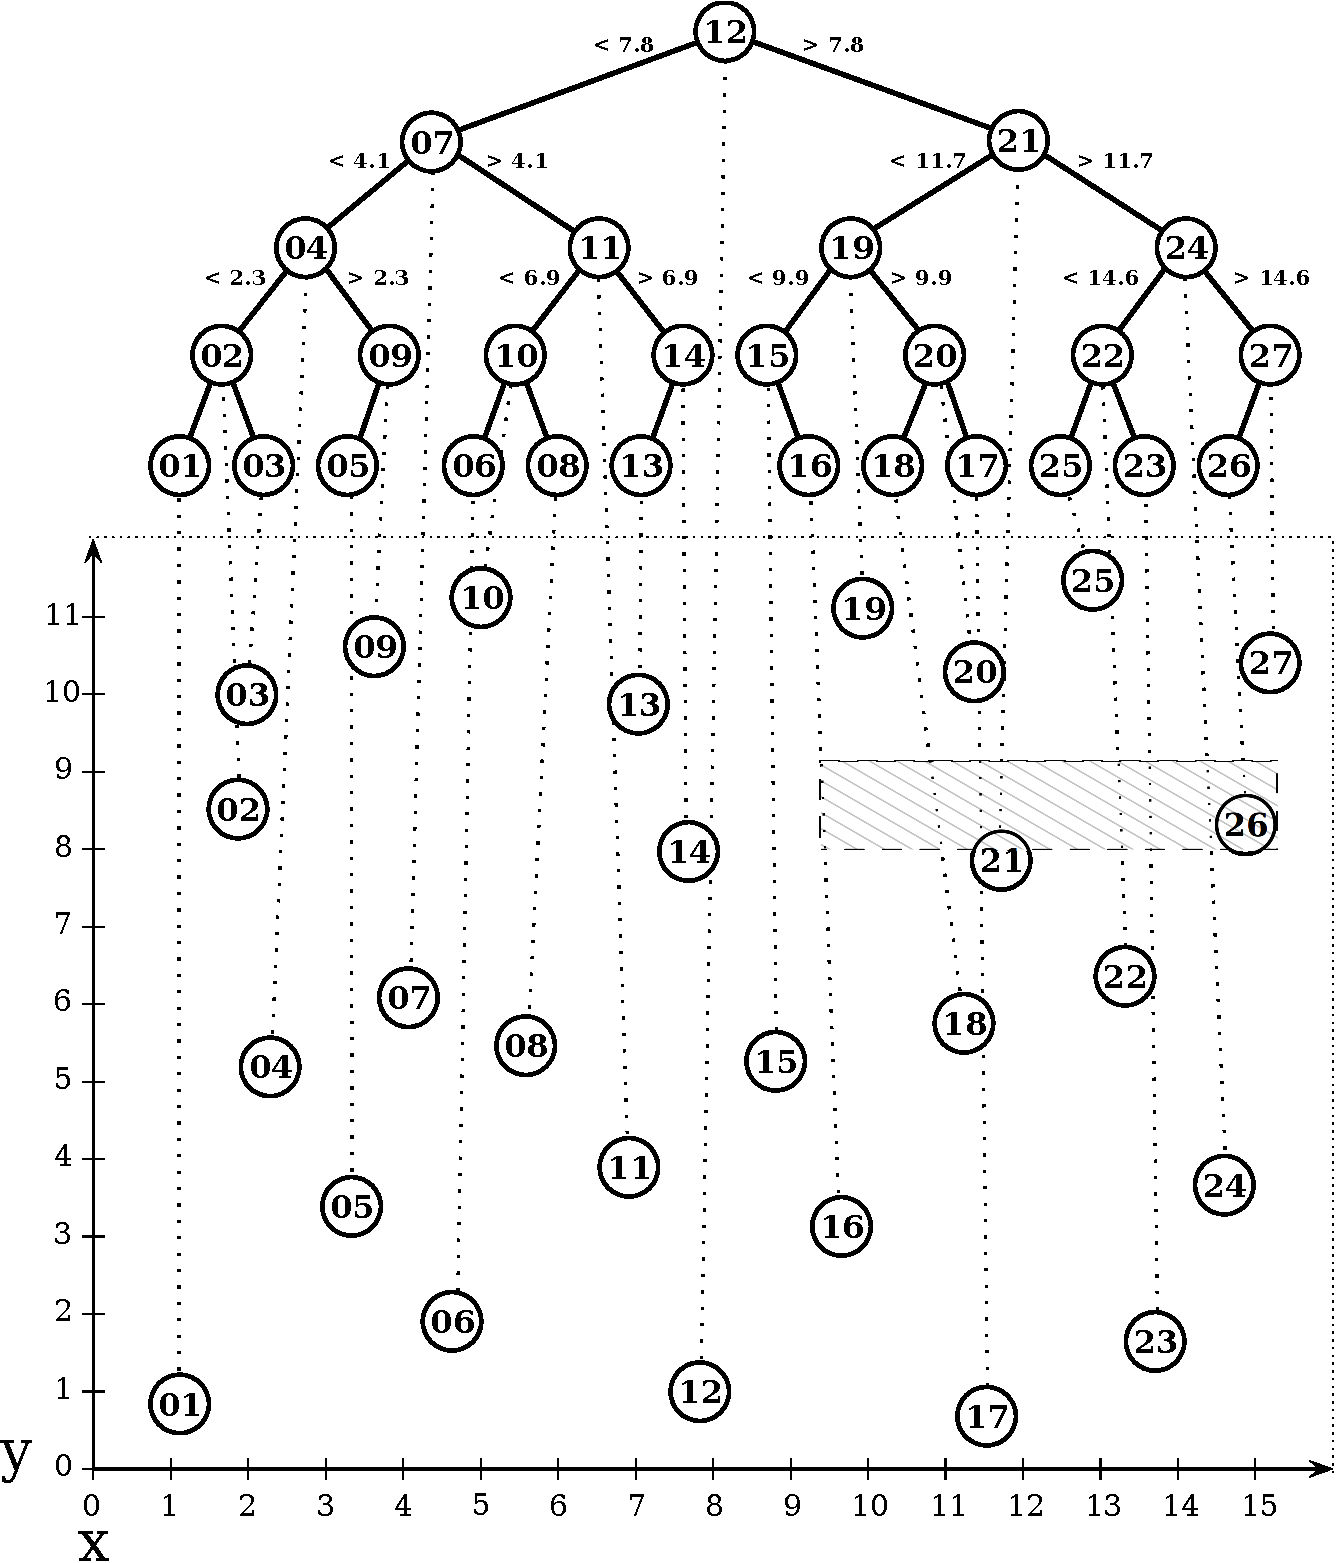
\includegraphics[width=\textwidth]{img/points-query/avl/points-avl-model}
    \caption{Pontos no plano mantidos por uma árvore AVL.}
    \label{img:pts-avl-model}
  \end{minipage}
  \hfill
  \begin{minipage}[t]{0.48\textwidth}
    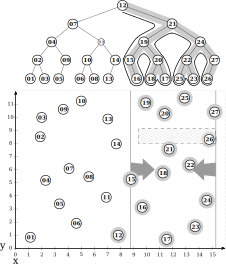
\includegraphics[width=\textwidth]{img/points-query/avl/points-avl-query}
    \caption{Execução da operação de busca de faixa em pontos mantidos por uma árvore AVL.}
    \label{img:pts-avl-query}
  \end{minipage}
\end{figure}



\section{\Kdtree{}}

Proposta por Jon Louis Bentley em~\cite{bentley1975}, a \kdtree{} é um tipo de
árvore binária de construção simples e baixa utilização de memória.
Devido a sua simplicidade e eficiência em indexação multidimensional,
é uma das estruturas mais utilizadas para operações de verificação de pertinência
multidimensional, como é o caso da busca de faixa~\cite{preparata2012computational}.
Além da operação de busca de faixa, a \kdtree{} suporta outras operações como busca de vizinho mais próximo, e por isso é também utilizada em algoritmos de
clusterização~\cite{kanungo2002efficient, indyk1998approximate}
e renderização gráfica~\cite{owens2007survey}.

Como qualquer árvore binária, cada nível recursivo da
\kdtree{} subdivide os dados em duas partes, porém, ao invés de utilizar
apenas uma \emph{chave} em todos os níveis da árvore, a \kdtree{} utiliza um
total de $k$ chaves, fazendo um revezamento circular entre as chaves, à medida
que caminha nos níveis da árvore.
Dessa forma, os elementos do 1º nível da árvore consideram como chave
a 1ª dimensão,
o 2º nível da árvore considera a 2ª dimensão, o $k$º nível considera a $k$ª dimensão,
o $k+1$º nível considerada a 1ª dimensão, e assim por diante.

Com relação à eficiência da \kdtree{} é importante considerar que não é
recomendável escalar de forma arbitrária o número $k$ de dimensões
indexadas pela \kdtree{}, esperando assim escalar também sua eficiência,
mesmo no caso de dados  definidos em muitas dimensões.
Como regra geral considera-se que uma \kdtree{} é adequada para indexar um
conjunto com $n$ pontos se $n$ não for muito maior que $2^k$~\cite{toth2004handbook},
caso contrário, a performance da \kdtree{} se assemelhará a de uma busca
linear exaustiva, como em uma lista encadeada.

A Figura~\ref{fig:kdom-kd} apresenta um conjunto de pontos dispostos num
espaço bi-dimensional (a) e indexados por uma \dtree{2} (b).
O primeiro e terceiro nível da \dtree{2} indexa a componente $x$ dos pontos,
enquanto o segundo nível indexa a componente $y$.
Cada ponto indexado pela árvore subdivide o espaço em dois de acordo
com o valor da componente que está sendo indexada.
A subdivisão do espaço é representada na figura por uma linha mais grossa.

\begin{figure}
  \centering
  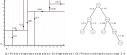
\includegraphics[scale=4.8]{img/kdt/dom-kd}
  \caption{Exemplo de pontos indexados por uma \kdtree{}.}
  \label{fig:kdom-kd}
\end{figure}

A Figura~\ref{img:pts-kdt-model} apresenta os mesmos 27 pontos e
área de busca (retângulo pontilhado) das Figuras~\ref{img:pts-lst-model},
\ref{img:pts-lst-query}, \ref{img:pts-avl-model} e \ref{img:pts-avl-query},
porém agora os pontos estão mantidos por uma \kdtree{} indexando as componentes
$x$ e $y$.
Os 1º, 3º e 5º níveis da árvore dividem o plano segundo o valor da componente $x$
enquanto os 2º e 4º níveis dividem o plano segundo o valor da componente $y$.

A Figura~\ref{img:pts-kdt-query} ilustra a operação de busca de faixa utilizando
a árvore k-d.
As setas acinzentadas no plano indicam a direção da varredura, executada após
a avaliação do ponto responsável pela indexação das regiões em questão.
Os pontos avaliados na operação estão marcados com um fundo circular acinzentado.
As setas junto à árvore na parte superior da figura indicam a ordem em que os
pontos foram avaliados.
Para iniciar a operação de busca de faixa utilizando a \kdtree{} é necessário
observar os limites tanto no eixo $x$ quanto em $y$ do retângulo de busca.
Inicialmente avalia-se a possível pertinência da região de busca em ambos os
planos divididos verticalmente pelo ponto 15.
Como a região de busca não possui intersecção na região à esquerda do ponto 15
($x < 8.8$),
toda essa região é descartada e o algoritmo segue para a região à direita do plano ($x \geq 8.8$),
a qual é indexada verticalmente pelo ponto 22.
Como a região inferior ao ponto 22 ($y < 6.4$) não possui intersecção com a
área de busca, o algoritmo descarta essa região inferior e segue para avaliar a
região superior ($y \geq 6.4$), a qual é indexada horizontalmente pelo ponto 25.
Como ambas as regiões separadas pelo ponto 25 possuem intersecção com a
área de busca, o algoritmo deve considerar ambas as regiões, escolhendo uma
delas para avaliar primeiro.
O algoritmo segue realizando as avaliações de forma sucessiva
até encontrar o ponto 26, pertencente à região de busca.
Na operação foram avaliados $6$ dos $27$ pontos.
Caso o algoritmo desse prioridade à região a direita do ponto 25,
apenas $4$ pontos seriam avaliados.

\begin{figure}[ht]
  \centering
  \begin{minipage}[t]{0.48\textwidth}
    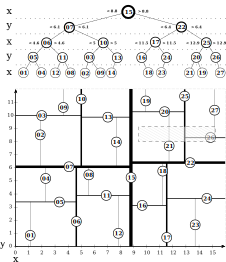
\includegraphics[width=\textwidth]{img/points-query/kdt/points-kdt-model}
    \caption{Pontos no plano mantidos por uma árvore k-d.}
    \label{img:pts-kdt-model}
  \end{minipage}
  \hfill
  \begin{minipage}[t]{0.48\textwidth}
    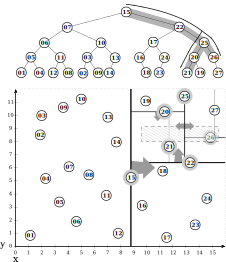
\includegraphics[width=\textwidth]{img/points-query/kdt/points-kdt-query}
    \caption{Execução da operação de busca de faixa em pontos mantidos por uma árvore k-d.}
    \label{img:pts-kdt-query}
  \end{minipage}
\end{figure}

Outra estrutura que suporta a operação de busca de faixa em casos bidimensionais é a quadtree,
árvore proposta por Finkel e Bentley em~\cite{finkel1974quad}
e frequentemente utilizada em processamento de imagens~\cite{de1997computational} e geração de malhas~\cite{cheng2012delaunay}.
A quadtree é uma árvore que divide o espaço em quadrantes.
No caso bi-dimensional, por exemplo, cada nó da árvore possui até quatro sub-árvores filhas, representando os 4 quadrantes
que fazem interseção com o respectivo ponto.
Dessa forma, os nós de uma quadtree que indexa $k$ dimensões possuem até $s^k$ sub-árvores filhas.
Segundo a literatura, a utilização da quadtree para indexação de conjunto Paretos mostra-se eficiente
apenas em casos bi-objetivos de conjuntos Paretos extensos, acima de 15000 soluções~\cite{mostaghim2005quad}.
Conjectura-se que essa ineficiência é decorrente do alto \emph{overhead} da estrutura, especialmente para os casos com mais de dois objetivos.

Espera-se que a \kdtree{} auxilie as operações de verificação de dominância
ao descartar uma grande quantidade de soluções, demandando um menor número
de comparações entre soluções, melhorando assim a performance dos algoritmos.
Infelizmente não se tem uma análise formal de complexidade da busca de faixa
utilizando a \kdtree{}. Segundo Bentley, a versatilidade da busca de faixa
utilizando a \kdtree{} torna sua análise formal extremamente difícil~\cite{bentley1975}.

\missingf{Acho que seu capítulo de principal contribuição tá com pouco conteúdo!!!
Vc compara a kd-tree com lista encadeada e AVL-tree porque foram as estruturas usadas pela Bazgan. Mas, a estrutura de dados nao era o foco do trabalho da Bazgan.
Conjecturo que nao estava interessada em propor algo nesta area. Provavelmente usou lista e AVL apenas por ser de facil implementacao.
Acho que precisa ter uma discussao em cima disso e se teriam outras estruturas 
que tb poderiam ser usadas.
Acho que vc tambem deveria reconsiderar a possibilidade de fazer uma análise de complexidade aqui. Isso daria uma robustez teórica maior ao seu trabalho!!!
}